\section{Application case: RadarBot}
	\par \textbf{RadarBot: Speed Camera Detector } is an Android application able to retrieve data about traffic and speed cameras while driving. It counts more than 50 millions downloads on Google Play and it is the first application analyzed of the \textit{Navigation \& Maps} category in this study. This application will notify the user about every alert regarding the driving and for this reason it requires a constant interaction between mobile app and the server delivering the service. 
	
	\subsection{Study detail}
		\par Once installed RadarBot and started the application for the first time, the user is asked to register a new account though the Google or Facebook identity providers. In this application case the user cannot register a new account without having completed this step, so I proceeded with linking my personal Google account. At this point the account is created, and the application is ready to use. The application starts with the visualization of our current position on a map. \newline
		\par The first tool used to inspect the application behaviour is \textit{HttpToolkit}. The application interacts with different enpoints using the HTTPS protocol, that means every request is encrypted, but since we placed our proxy tool in the middle of the communication we are still able to investigate the application behaviour. Most of the requests are directed towards two endpoints:
		\begin{enumerate}
			\item \textbf{clients4.google.com}: This is the endpoint relative to the GoogleMaps API used in this application to retrieve the portion of map to display in the application. Since the user will constantly change position while driving, lots of this kind of request will be issued to retrieve the map. In any case the data contained in the response is only related to the representation of the map itself (streets and buildings).
			\item \textbf{radarbotservices.com}: This is the real server delivering the RadarBot services. Multiple POST requests are done on different resources.
		\end{enumerate}
		Among the other requests we can notice the \textit{OneSignal} notification service and the \textit{Firebase} logging service (same for \textit{iLMeteo} application).
		
		\subsubsection{RadarBotServices requests}
			\par \textit{radarbotservices.com} is the endpoint responsible for delivering most of the feature implemented in the application, for example the alerts delivery system or the possibility to create a new alert on the map. \newline
			\par The first request issued while using the application is a POST on the resource called \textbf{ws\_check\_update\_database.php}. In the body of the request we can notice the \textit{device\_id} and the \textit{firebase\_id}. Probably this is the request responsible of notifying the server that the device is using the RadarBot service, and at the same time the version of the software is checked. As response we got a simple \textit{"code": 0,"message": "WS OK","new\_version": 1} message.\newline
			\par Right after a new POST request is issued on the resource \textbf{ws\_get\_licence.php}. As before the body request contains \textit{device\_id} and \textit{firebase\_id}. In the response this time we get some identifiers relatives to the licences used by the application. In fact RadarBot offers either a free or a premium service. With this request the application is checking if a premium licence is active on our device.\newline
			\par At this point the application will update the information on the user using RadarBot. Therefore another POST request is issued towards \textbf{ws\_user.php} sending again in the body again informations on  \textit{device\_id} and \textit{firebase\_id}, but also private informations such as \textit{latitude}, \textit{longitude} and \textit{email}. The response message received is \textit{"code": 0,"message": "User updated OK"}.\newline
			\par The above described requests are done in the initialization phase of the application. After this setup, the application behaviour enters a loop where two requests are repeatedly issued. \newline
			The first request is a POST on \textbf{ws\_get\_country.php} where the application notify the server of some movement, if happened. In the body there are both \textit{latitude} and \textit{latitude} coordinates. The response will contain the country where we currently are. The message is \textit{"code": 0,"country\_code": "it"}. \newline
			The second is request is another POST on \textbf{ws\_get\_alerts.php} where the informations regarding speed cameras and alerts are retrieved by the client. Even in this case the \textit{latitude} and \textit{longitude} coordinates are sent to the server. The response is depending on the alerts database. In the pictures above there is an example:
			\begin{figure}[ht]
				\centering
				\subfigure[Radarbot application response view]{
				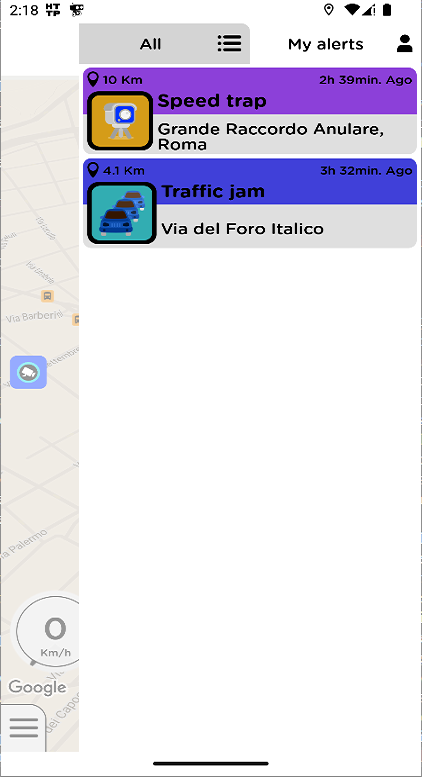
\includegraphics[width=.45\textwidth]{images/radarbot_alerts1.png}
				}
				\subfigure[HTTPS response]{
				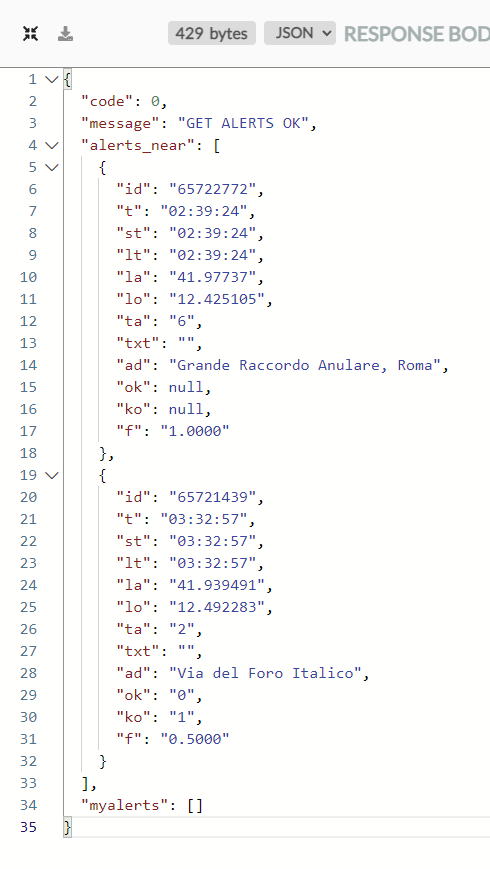
\includegraphics[width=.45\textwidth]{images/radarbot_alerts2.png}
				}
				\caption{Retrieving alerts in RadarBot application}
				\label{radarbot_alert}
			\end{figure}
			\par As you can see in this example there are two items in the \textit{alerts\_near} list. The first one is relative to the alert on \textit{Grande Raccordo Anulare}, while the second one is relative to the alert in \textit{Via del Foro Italico}. Informations on the alerts are comprehensive of \textit{alert\_id}, \textit{latitude}, \textit{longitude} and \textit{time} since report.\newline
			
			\par Since we are interested in user informations, the application investigation continues looking for any evidence of user ids. After having checked some other less relevant requests (like the ones generated when rating alerts on the map, creating an alert or removing an alert), we notice that there are no informations on any other user of the Radarbot service. The only information exchange at which the client takes part are the one related to itself.
		
	\subsection{Sensitive data}
		\par In terms of sensitive and private data, the informations involved in the communication protocol are:
		\begin{itemize}
			\item \textbf{device id}: It is present in the body field of each requets generated.
			\item \textbf{firebase id}: It is used as actual user id for every request. At this id are associated also information on the device (hardware, device model, os build)
			\item \textbf{latitude and longitude}: As described in the previous section, these fields are sent in the requests \textit{ws\_get\_country} and \textit{ws\_get\_alerts}.
			\item \textbf{email}: The user email is sent in the request \textit{ws\_user} in the initialization phase of the application.
		\end{itemize}
		\par All these information are related to the user currently using the RadarBot application. In any case the communication flow is encrypted by the use of the HTTPS protocol, so every discussed information is obscured to third parties. The presence of a Man-In-The-Middle, and therefore of a proxy installed on the device redirecting the traffic to a controlled server, is still able to retrieve the informations above.\newline
		\par No private informations are available on the other users of the Radarbot service.
		
	\subsection{Other vulnerabilities}
		\par While looking for any information user related in the network communication flow, some specific behaviour of the application have been investigated. For example the possibility to remove alerts from the map created by some other user. \newline
		\begin{figure}[ht]
			\centering
			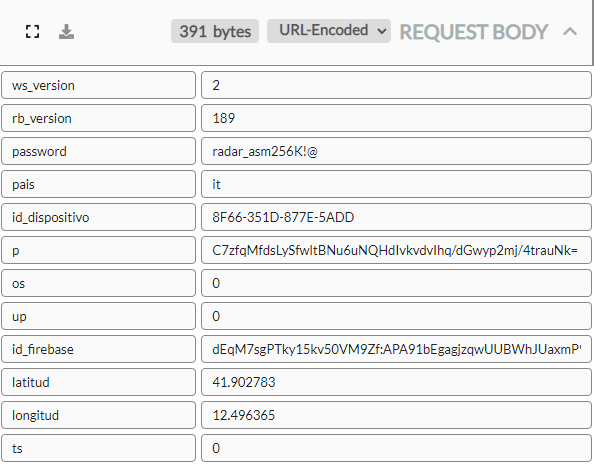
\includegraphics[width=0.9\textwidth]{images/radarbot_request.png}
			\caption{Radarbot body request fields.}
		\end{figure}
		\newpage
		\par From this point of view the application relies on two variables that are present in the body of each request generated by the client, showed in the picture above. The first one is \textit{id\_firebase} that is evaluated as actual user id. The second one is the \textit{p} field containing a Base64 value sent in each request. \newline
		In the case in which the \textbf{id\_firebase} field is not sent in the body, the request is ignored, obtaining a void response from the server. \newline
		On the other side, if the \textbf{p} field is not sent in the body, the related response will contain the message \textit{"code": 2,"message": "BBDD PARAMS WS"}. \newline
		\par In order to test any other vulnerability affecting the application is needed to forge a request that will be accepted by the server, and then we need to forge a new value for the field \textit{p}.
		
		\subsubsection{Forging requests}
			\par In order to forge any valid request, the field \textbf{p} has to be set accordingly. Starting analyzing two identic requests on the same path (same headers, same body values), the field \textit{p} assumes two different values. \newline
			\par In order to inspect how this field is computed at runtime I gave a look at the source code of the application using the tool \textit{GDA}. By a searching the string \textit{''id\_dispositivo''} I rapidly came up into the piece of code where the body fields are taken into account: This is the code:
			\begin{figure}[ht]
				\centering
				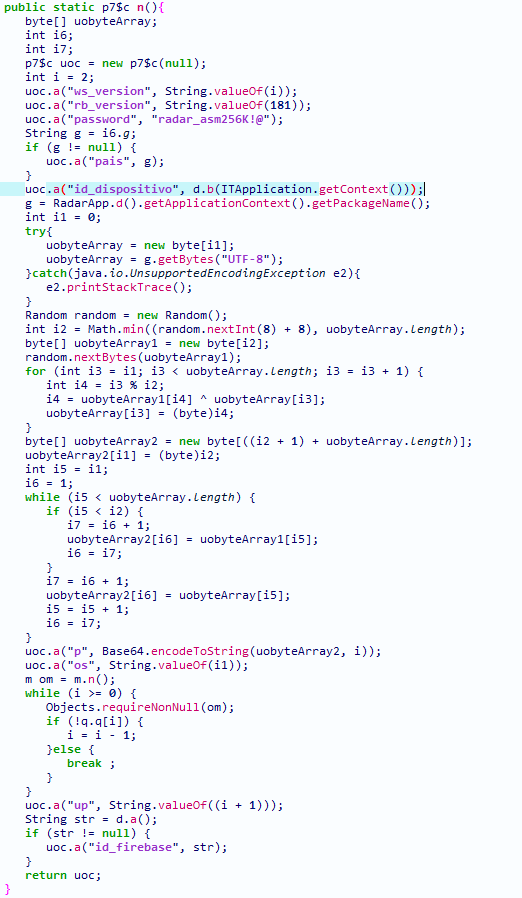
\includegraphics[width=0.9\textwidth]{images/radarbot_gda.png}
				\caption{Radarbot source code method.}
			\end{figure}
			\par The highlithed line shows the string searched. As we can see there are all the main fields of the body: \textit{ws\_version}, \textit{rb\_version}, \textit{password}, \textit{pais}, \textit{id\_dispositivo}, \textit{p}, \textit{os}, \textit{up}. Specifically the field \textit{p} seems to be computed starting from the bytes of the string relative to the RadarBot package name. Random values are then computed and integrated in some way in the byte array. At the end the value obtained is encoded in Base64 and assigned at the field \textit{p}.\newline
			\par At this point we know exactly how the \textit{p} value has been computed. In order to generate more valid values I created a Java program with the same line codes relative to the computation of this value. The code is omitted since it is just a copy-paste from the source code with some adjustment. In this way we are able to compute an infinite amount of values for the variable \textit{p}.   \newline
			Notice that the only values that contributes to the final value of \textit{p} are: the package name (\textit{''com.vialsoft.radarbot\_free''}) and some integer values fixed or computed at runtime from random values. \newline
			\par By changing the field \textit{p} of some already working requests with the value generated by our Java program, the requests are being accepted, meaning that our program is working and generating good values for the field \textit{p}. In particular there is no time-relative constraint on this value, meaning that once obtained one it can be reused an infinite amount of time. \newline
			\par Regarding to the \textbf{firebase\_id} value there is nothing we can do. It is an user id assigned by the Firebase service, and the RadarBot server uses it as user id. 
			
		\subsubsection{Test: remove other users alerts}
			\par Now that we are able to manually forge requests, the investigation continues on testing some edge cases. For example the case in which an user request to remove an alert created by another user. We already have seen in Picture \ref{radarbot_alert}, how an alert identifier can be retrieved while using the application. \newline
			When the user asks to remove an alert that he himself created, a new POST request is issued on the path \textbf{ws\_remove\_alert.php}. Another value has to be added in the body that is \textit{id\_alerta}, representing the id of the alert that the user wants to delete. This is the forged request and the relative response, obtained using the \textit{Repeater} tab from the \textit{BurpSuite} tool:
			\begin{figure}[ht]
				\centering
				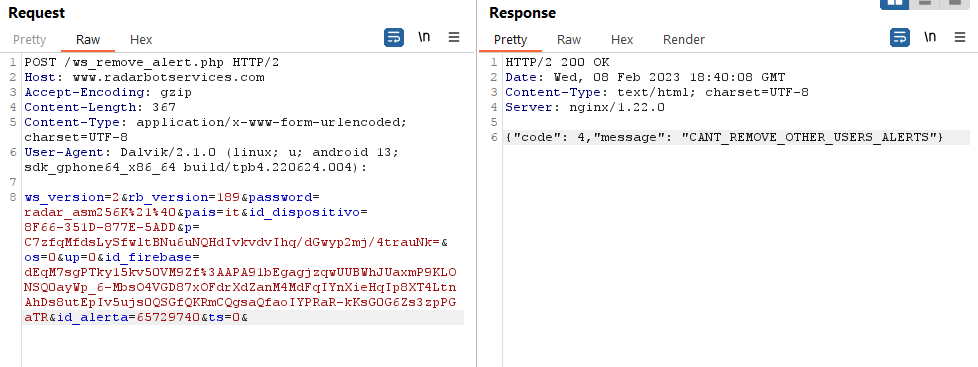
\includegraphics[width=0.9\textwidth]{images/radarbot_removealert.png}
				\caption{Forged remove alert request and response.}
			\end{figure}
			\par As you can see the request is accepted by the server, but the response shows the message \textit
{"code": 4,"message": "CANT\_REMOVE\_OTHER\_USERS\_ALERTS"}. So the server is recognizing that the alert has not been created by the user that requested the action, and it is blocking the action.

		\subsubsection{Test: modifying user informations}
			\par Another vulnerability check has been conducted on the request \textbf{ws\_user} where the client communicates the update relative to a user profile. For example a possible request might be to modify the email relative to a user profile. In the picture below I tryed to change my personal email into the institutional email.
			\begin{figure}[ht]
				\centering
				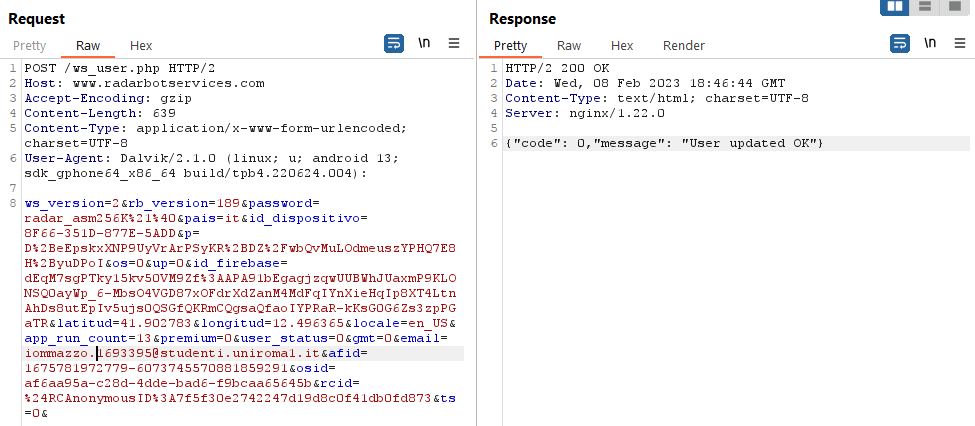
\includegraphics[width=0.9\textwidth]{images/radarbot_changeemail.png}
				\caption{Forged remove alert request and response.}
			\end{figure}
			\par Anyway in this case, even if the request is being accepted by the server showing the message \textit{"code": 0,"message": "User updated OK"}, there is no actual change in the server database or in the client application. In fact the email it is not changed, and the future request will still contain my personal email data.
			\newpage